\documentclass{article}
\usepackage{protools}

\addbibresource{towards.bib}

\setlength\parskip{0.25\baselineskip}

\begin{document}

\ArticleTitle
  {Towards Optical States Of Four Photons}
\ArticleAuthor*
  [0000-0002-5646-6964]
  {Jan Provazn\'{i}k}
  {provaznik@optics.upol.cz}
\ArticleAuthorAddress
  {Department of Optics, Palack\'{y} University, 17. listopadu 1192/12, 771 46 Olomouc, Czech Republic}

\ArticleAuthor
  {Olga Solodovnikova}
\ArticleAuthorAddress
  {Technical University of Denmark, Lyngby, Denmark}

\ArticleAuthor
  [0000-0002-5761-8966]
  {Petr Marek}
\ArticleAuthorAddress
  {Department of Optics, Palack\'{y} University, 17. listopadu 1192/12, 771 46 Olomouc, Czech Republic}

\ArticleAuthor
  [0000-0003-4114-6068]
  {Radim Filip}
\ArticleAuthorAddress
  {Department of Optics, Palack\'{y} University, 17. listopadu 1192/12, 771 46 Olomouc, Czech Republic}

\ArticleTitlePrint

\begin{abstract}\noindent
  Quantum non-Gaussian states and operations are a crucial component of quantum information processing protocols, but alas, both the realization of non-Gaussian operations for travelling modes of light and the preparation of non-Gaussian states pose significant practical challenges in contemporary experiments. In this paper, the minimal requirements imposed on the quantum efficiency of photon number resolving detectors and the quality of the squeezing operation in experimental realization of certifiable quantum non-Gaussian states of individual photonic states with three, four, and five photons.
\end{abstract}

% Introduction
%
%

\section{Introduction}

A measurement-based method for preparation of individual photonic states of light~\cite{yukawa2013a,yoshikawa2018,tiedau2019,provaznik2020} is discussed in the first section of this chapter. The mathematical model of the procedure takes loss into account, both in the construction of the state in during its characterization. The resulting states are certified using hierarchical criteria \cite{lachman2019} in the second section by evaluating the statistical behavior of the model under realistic experimental conditions. Figures presented in this section can be used to determine the minimal requirements on the efficiency of the optical components, such as squeezing and detection, in experimental realizations targeting states of two, three, and four photons.

% Methodology
%
%

\section{Cooking up states of travelling light}

Photonic Fock states can be conditionally prepared by using a two mode squeezed vacuum state and a photon number resolving detector~\cite{yukawa2013a,yoshikawa2018,tiedau2019,provaznik2020}. The theoretical model of the experimental scheme is illustrated in~\figref{f-scheme}. One of the entangled modes is measured, thus projecting the other mode onto the resolved Fock state. This procedure is repeated until a satisfactory detection outcome is observed; at that point the target state is successfully prepared. The outlined protocol assumes a perfectly squeezed state, lossless transmission and an ideal photon number resolving (PNR) detector. Some of the adverse effects of realistic inefficiencies can be effectively accounted for by considering lossy transmission of both modes prior to their measurement.

\begin{figure}[h]
  \begin{center}
    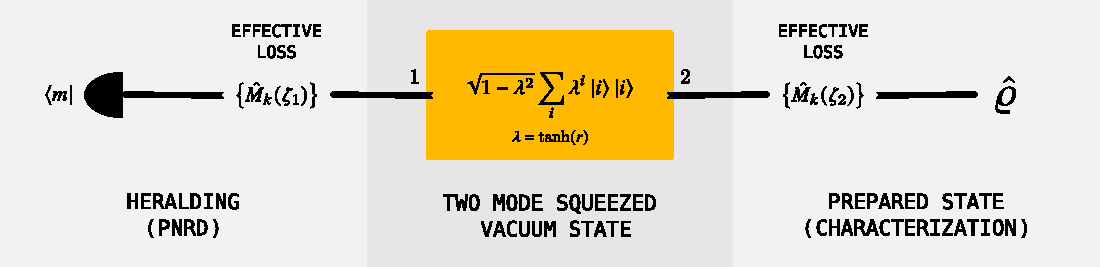
\includegraphics[width = 1.00 \columnwidth]{import/illustrate_scheme_alt.pdf}
  \end{center}
  \caption{
    Schematic illustration of the non-Gaussian state preparation circuit with a two mode squeezed vacuum state serving as a source of entangled quantum states. One of the modes is measured, thus projecting the other mode onto the resolved Fock state. A satisfactory detection outcome heralds a successful preparation of the target state. The outlined protocol assumes a perfectly squeezed state, lossless transmission and an ideal detector. Some of the adverse effects of realistic inefficiencies are accounted for by considering lossy transmission of both modes prior to their measurement.
  }
  \label{f-scheme}
\end{figure}


The resulting non-normalized marginal state is given by
%
\begin{equation}\label{e--rho}
  \hatrho_{(m)} \approx
  \sum_{i = 0}^{\infty} 
  \sum_{j = 0}^{\infty}
    \lambda^{i} \lambda^{j}
    \left(
      \sum_{k = 0}^{\infty}
        \bra{m} \hat{M}_{k} (\zeta_{1}) \ketbra{i}{j} \hat{M}_{k}^{\dagger} (\zeta_{1}) \ket{m}
    \right)
    \left(
      \sum_{k = 0}^{\infty}
        \hat{M}_{k}(\zeta_{2}) \ketbra{i}{j} \hat{M}_{k}^{\dagger} (\zeta_{2})
    \right) \Qc
\end{equation}
%
where $m$ identifies the detected Fock state, $\lambda = \tanh(r)$ characterizes the two mode squeezed state with initial squeezing $r$, and the Kraus operators $\hat{M}_{k} (\zeta) $ describe the transmission loss with
%
\begin{equation}
  \hat{M}_{k} (\zeta) =
    \sqrt{ \frac{(1 - \zeta)^{k}}{k!} } 
    \sqrt{\zeta}^{\hat{n}} \hat{a}^{k}
\end{equation}
%
where $\zeta$ gives the intensity transmittance of the lossy channel~\cite{ivan2011}. In the case of~\eqref{e--rho}, the parameter~$\zeta_{1}$ corresponds to loss in the first mode, called the heralding mode, whereas~$\zeta_{2}$ identifies the loss affecting the mode carrying the prepared state.

The probability of successful preparation, that is, the probability of detecting $m$ photons in the heralding mode, can be obtained analytically as
%
\begin{equation}\label{e-pnr-pro}
  P_{(m)} = (1 - \lambda^{2}) 
  \frac
    { (\lambda^{2} \zeta_{1})^{m} }
    { [ 1 - \lambda^{2} (1 - \zeta_{1}) ]^{m + 1} } \Qd
\end{equation}
%
The equation~\eqref{e--rho} for the resulting density matrix of the prepared state can be simplified. The matrix is diagonal in the Fock basis; its properly normalized elements are obtained as
%
\begin{equation}\label{e-pnr-rho}
  \braket{ k | \hatrho_{(m)} | k } =
  \frac
    { [ 1 - \lambda^{2} (1 - \zeta_{1}) ]^{m + 1} }
    { [ \lambda^{2} (1 - \zeta_{1}) ]^{m} }
  \left( \frac{ \zeta_{2} }{ 1 - \zeta_{2} } \right)^{k}
  H (k, m, x) \Qc
\end{equation}
%
where the substitution ${x \coloneqq \lambda^{2} ( 1 - \zeta_{1} )(1 - \zeta_{2} )}$ is used in the function $H(k, m, x)$ defined as
%
\begin{equation}\label{e--H}
  H(k, m, x) \coloneq
  \begin{dcases}
    \sum_{l = m}^{\infty}
      \binom{l}{m}
      \binom{l}{k}
      x^{l} 
    & k \leq m \Qc \\
    \sum_{l = k}^{\infty}
      \binom{l}{m}
      \binom{l}{k}
      x^{l}
    & k > m \Qd
  \end{dcases}
\end{equation}
%
The series in~\eqref{e--H} converge since ${\lambda^{2} ( 1 - \zeta_{1} )(1 - \zeta_{2} ) \leq 1}$. The infinite series in the formula can be alternatively expressed in terms of hypergeometric functions~\cite{bateman1981}, which are conveniently implemented in commonly available numerical libraries~\cite{virtanen2020}, leading to the expression
%
\begin{equation}
  H(k, m, x) \equiv
  \begin{dcases}
    x^{m} \binom{m}{k} {}_{2}F_{1} (1 + m, 1 + m, 1 + m - k, x)
    & k \leq m \Qc \\
    x^{k} \binom{k}{m} {}_{2}F_{1} (1 + k, 1 + k, 1 + k - m, x)
    & k > m \Qd
  \end{dcases}
\end{equation}
%
The model of state preparation, represented by relation \eqref{e--rho}, relies on ideal PNR detectors in the heralding stage of the circuit. While these detectors exist in principle \cite{hopker2019,endo2021,endo2024}, their practical availability is severely limited. The model of the experimental circuit can be extended to cover the more commonly available cascaded avalanche photodiode~(CAP) detectors~\cite{hlousek2019,grygar2022,hlousek2024,ercolano2024} with capacity to approximate actual PNR detectors, especially in the context of state preparation~\cite{provaznik2020}.

The incoming signal is divided equally between $n$ independent avalanche detectors comprising the cascade. The detection events when $m$ out of the $n$ constituent detectors become triggered, that is, register any positive number of photons, are associated with the elements~\cite{paul1996}
%
\begin{equation}\label{e-capd}
  \begin{gathered}
  \hat{\Pi}_{m}^{n} 
    \coloneqq \sum_{k = 0}^{\infty} w(k, m, n) \ketbra{k}{k} \\
  \text{where} \quad
  w(k, m, n) 
    \coloneqq 
    \begin{dcases}
      \; \frac{1}{n^{k}} \binom{n}{m} \sum_{l = 0}^{m} \binom{m}{l} (-1)^{l} (m - l)^{k} 
      & \text{when}\quad k \geq m \\
      \; 0 & \text{otherwise} \Qd
    \end{dcases}
  \end{gathered}
\end{equation} 
%
The number of detectors in the cascade must be sufficiently high to minimize the probability of individual detectors registering multiple photons. Consequently, ideal PNR detectors are well approximated only in the limit of very large number~$n$ of the constituent avalanche detectors~\cite{provaznik2020}.

Adaptation of the relations \eqref{e-pnr-pro} and \eqref{e-pnr-rho} to the use of CAP detectors is rather straightforward. The probability of success when post-selecting on the $\Pi_{m}^{n}$ outcome, that is, when $m$ detectors out of $n$ register photons, is the weighted average of the individual probabilities,
%
\begin{equation}\label{e-cap-pro}
  P_{(m, n)} = \sum_{k} w(k, m, n) P_{(k)} \Qc
\end{equation}
%
as the elements \eqref{e-capd} of CAP detectors are diagonal in Fock basis. Similarly, the resulting density matrix remains diagonal. It is also a weighted average of the individual matrices,
\begin{equation}\label{e-cap-rho}
  \hatrho_{(m, n)} =
    \frac{1}{P_{(m, n)}}
    \sum_{k} w(k, m, n) 
      P_{(k)} \hatrho_{(k)}
  \Qd
\end{equation}

% Certification
%
%

\section{Certifiable quantum non-Gaussian states}

One of the major experimental challenges in preparation of quantum states of light is the omnipresent loss and noise. It diminishes quantum correlations between entangled resources and reduces the quantum efficiency of detectors, making it impossible to prepare the desired quantum state with perfect fidelity. The reduced detection efficiency affects both the preparation of the quantum state and its subsequent characterization. This additional uncertainty can be partly alleviated using bespoke criteria for certification of genuine $m$-photon quantum non-Gaussian states~\cite{lachman2019} offering a certain degree of robustness against loss incurred during state characterization while also requiring only partial information about the tested state.

A quantum state which can not be decomposed into a statistical mixture of pure states attainable by Gaussian transformations of superposed Fock states up to ${\ket{m - 1}}$ is called a genuine $m$-photon quantum non-Gaussian ($m$-PQnG) state~\cite{lachman2019}. This is closely related to its stellar rank~\cite{chabaud2020,fiurasek2022}. It is possible determine whether a state $\hatrho$ belongs to specific $n$-photon hierarchy by examining a relationship between its first $n$ Fock state contributions,
%
\begin{equation}
  x_{m} 
    = 1 - \sum_{k = 0}^{m - 1} 
      \braket{k | \hatrho | k}
  \quad\text{and}\quad
  y_{m} = \braket{m | \hatrho | m}
  \Qd
\end{equation}
%
The state is a genuine $n$-PQnG state when ${y_{m} \geq F_{m} (x_{m})}$. The threshold function $F_{m}(x)$ can be obtained by means of sophisticated numerical optimization \cite{lachman2019,fiurasek2022}.

% Monte Carlo Simulation
%
%

\subsection*{Monte Carlo simulation of the state preparation circuit}

The relations~\eqref{e-pnr-rho}~and~\eqref{e-cap-rho} provide the diagonal elements of the conditionally prepared quantum state, depending on the choice of heralding detectors used in the experiment. These relations are functions of the initial squeezing rate~$r$, the losses~$\zeta_{1}$ and~$\zeta_{2}$ incurred in both modes, and the post-selection imposed on the measurement outcome $m$. The maximal tolerable amount of loss in the circuit capable of preparing a certifiable genuine~$m$-PQnG state can be determined by numerically simulating the experiment. The measurement statistics of a realistic experiment can be emulated using a Monte Carlo simulation based on the theoretical model of the circuit. 

The choice of the detectors does not affect the methodology of the simulation and the subsequent state certification. Without a loss of generality the following description is given in terms of the simpler relation~\eqref{e-pnr-rho}.

The preparation circuit is simulated for different amounts of loss $\zeta_{1}$ and $\zeta_{2}$ in both modes, varying initial squeezing rates $r$ and target states~${m}$. Detection events in the simulated experiment are drawn as random samples from a multinomial distribution bootstrapped with the diagonal elements $\braket{k|\hatrho_{(m)}|k}$ (where $0 \leq k < 20$) of the computed density matrix~\eqref{e-pnr-rho}. 

The number of random samples reflects the probability of successful preparation $P_{(m)}$. The probability \eqref{e-pnr-pro} depends on the initial squeezing rate and the loss in the heralding mode. Given a budget of $10^{8}$ repetitions available in a single realistic experimental run, only ${\lfloor 10^{8} \times P_{(m)} \rfloor}$ samples are drawn from the distribution. The samples are used to estimate the experimental probability distribution ${\overline{p}_{k} \approx \braket{k|\hatrho_{(m)}|k}}$. This random process is repeated to obtain $1000$ independent experimental runs for the subsequent statistical analysis.

Certification of the prepared states is achieved with the hierarchical criteria~\cite{lachman2019}. 
%
The estimated experimental probabilities $\overline{p}_{k}$, obtained in each simulated run of the experiment, are used to compute the aggregate random variables
%
\begin{equation}
  x_{m} = 1 - \sum_{k = 0}^{m} \overline{p}_{k} 
  \quad\text{and}\quad
  y_{m} = \overline{p}_{m} 
  \Qd
\end{equation}
%
Their expectation values $\mu_{x_{m}}, \mu_{y_{m}}$ and standard deviations $\sigma_{x_{m}}, \sigma_{y_{m}}$ are then used to certify the quantum state resulting from the simulation with the particular choice of $(m, \zeta_{1}, \zeta_{2}, r)$ parameters. The experimental state is considered to be certifiably genuine $m$-PQnG state if the expectation values lie at least three standard deviations away from the threshold function~$F_{m} (x)$. The operating principle of the certification procedure is illustrated in~\figref{f-otm-il}.

%

\begin{figure}[h]
  \begin{center}
    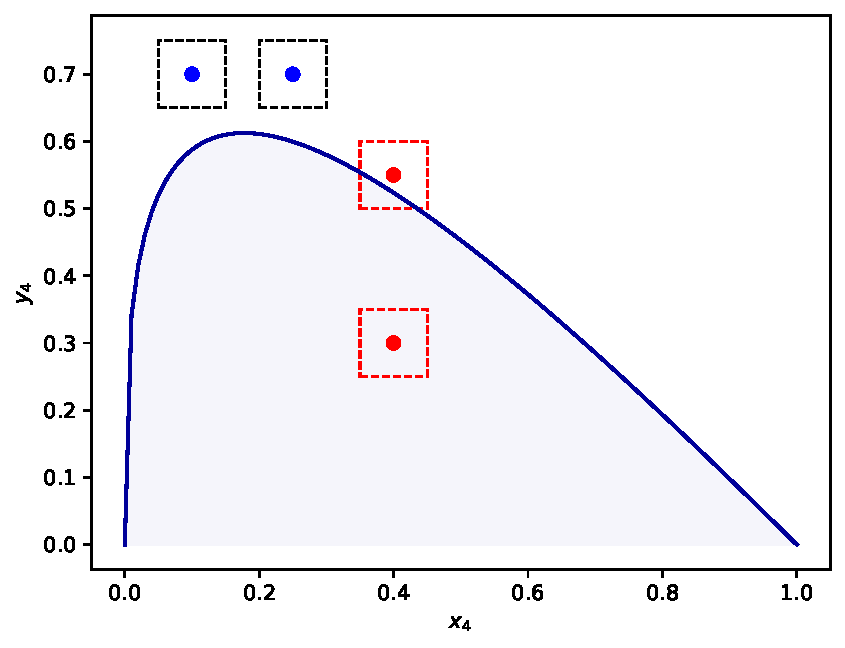
\includegraphics[width = 0.50 \columnwidth]{import/illustrate_lachman_curve.pdf}
  \end{center}
  \caption{
    Illustration of the certification procedure. The blue line represents the threshold curve $F_{4} (x)$. States with $y_{4} > F_{4}(x_{4})$ are genuine $4$-PQnG states. Four example experimental states are depicted in the figure. The bullet points represent their expectation values, $\mu_{x_{4}}$ and $\mu_{y_{4}}$, obtained by simulating the experiment. The dashed boxes represent their uncertainty and would normally span three standard deviations, $\sigma_{x_{4}}$ and $\sigma_{y_{4}}$, in each respective dimension. The pictured boxes are exaggerated in size for legibility of the illustration. States marked with red bullets failed the certification as they lie either under the threshold curve or their respective uncertainty boxes intersect the curve. States marked with blue bullets are certifiably genuine $4$-PQnG states according to the criteria; their boxes are well above the curve and do not intersect the curve.
  }
  \label{f-otm-il}
\end{figure}

% Results
%
%

\FloatBarrier
\section{Discussion of results}

In each dataset related to the tuple $(m, \zeta_{1}, \zeta_{2})$ of parameters the maximal probability of success is found with respect to the squeezing rate ${r \leq 10\,\dB}$. Both the maximal probability $P_{m}^{\star}$ and the respective optimal squeezing rate ${r^{\star}}$ are visualised in a grid as functions of ${(1 - \zeta_{1}, 1 - \zeta_{2})}$ for each target state $m$. In addition, to present only statistically significant results in the visualisation, grid cells where the probability of success lies below a reasonable threshold set to $10^{-5}$, which guarantees at least $1000$ successful realizations of the state within each experimental run, were blanked out.

The achievable success rate in preparation and subsequent certification of genuine $m$-photon states is presented in~\figref{f-otm-234}. Each column pertains to the particular target state $m = 2, 3, 4$. The maximal probabilities of success $P_{m}^{\star} (1 - \zeta_{1}, 1 - \zeta_{2})$ are presented in the top row, whereas the corresponding optimal squeezing rates $r^{\star} (1 - \zeta_{1}, 1 - \zeta_{2})$ are provided in the bottom row.
To reflect on the experimental limitations, the optimization is constrained to squeezing rates limited by $10\,\dB$. The figure also effectively shows the amount of loss that can be tolerated in the experiment.

In the case of the $2$-photonic state the tolerable loss exceeds $40\%$ in both modes. The probability of success ranges from roughly $10\%$ to $0.1\%$. The higher the loss, the lower the optimal squeezing rate. The tolerable loss is much lower for the state with $3$ photons. The maximal probabilities of success are also reduced. If the state suffers $40\%$ loss during preparation, it can only tolerate at most $20\%$ loss in its characterization. Higher loss leads to success rates lower than the $10^{-5}$ threshold  set earlier; the information obtained in the blanked out region is assumed to be unreliable. Finally, the conditions for the 4 photon state are even less favorable; while it is still possible to tolerate up to $40\%$ loss during preparation, the limit on $1 - \zeta_{2}$ is much more stringent, only about $10\%$ loss is permitted.

The two mode squeezed vacuum state is assumed to be ideal. The photon number resolving detectors are also presumed to be perfect with unit quantum efficiency. In realistic experiments these assumptions are never true, however, both the inefficiencies in detection and preparation of the squeezed state can be modeled with loss. Consequently the presented results cover these imperfect cases as well since any loss in the initial squeezed state generation are subsumed in the detection losses.

\begin{figure}[h]
  \begin{center}
    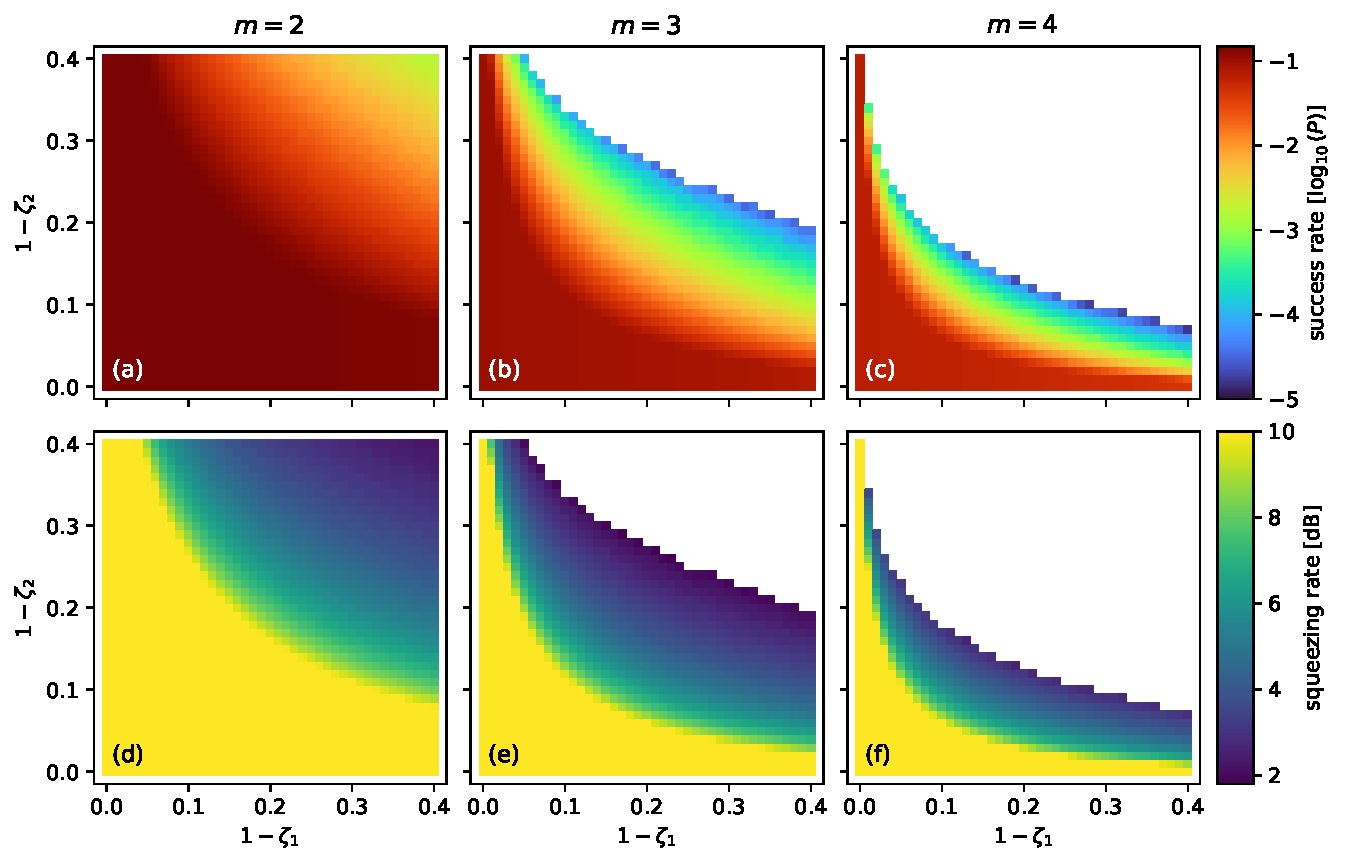
\includegraphics[width = \columnwidth]{import/hierarchy_2-3-4_1000.pdf}
  \end{center}
  \caption{
    The tolerable loss in preparation and subsequent certification of genuine $m$-photon states. Results for target states $m = 2, 3, 4$ are shown in columns. The maximal probabilities $P_{m}^{\star}$ of successful preparation of the certifiable target state, given the particular combination of loss $1 - \zeta_{1}$ incurred during preparation and the loss $1 - \zeta_{2}$ affecting the certification, are presented using a logarithmic scale in the top row. The optimization is constrained to squeezing rates limited by $10\,\dB$. The respective optimal squeezing rates $r^{\star}$ are provided in the bottom row.
  }
  \label{f-otm-234}
\end{figure}

% Conclusions
%
%

\FloatBarrier
\section{Conclusions}

The results presented in this chapter offer an insight into feasible experimental preparation of certifiable genuine $m$-photon states for $m = 2, 3, 4$. While preparation of quantum states of travelling light of up to three photons has already seen its experimental realization~\cite{yukawa2013a}, the construction of a $4$-photon state of travelling light still remains an open problem that will perhaps benefit from the analysis.

% References
%
% 

\FloatBarrier
\printbibliography[heading = bibnumbered]

\end{document}

% vim: linebreak breakindent breakindentopt=shift\:-2 showbreak=↳\  syntax=tex colorcolumn=
